% !TEX root = ../../main.tex

% Reset graphics to the current folder
\graphicspath{ {\thisch/figures/} }

\chapter{Appendix for \autoref{pyg}}%
\label{appx:pyg}


\section{Installation details for pyGAPS}

The source code for the framework is available at GitHub
at \url{https://github.com/pauliacomi/pyGAPS}. A highly detailed 
manual can be accessed through readthedocs
at \url{https://pygaps.readthedocs.io}
The PyPi distribution of the latest stable version can be found at
\url{https://pypi.org/project/pygaps}
or installed automatically through pip using \lstinline{pip install pygaps}.

\section{Further pyGAPS examples}\label{appx:pyg:examples}

\subsection{The generic isotherm print function}

\begin{python}[caption={Generic info function},label={appx:lst:print_info}]
isotherm.print_info()
\end{python}
\begin{pythonout}
Experimental isotherm
Material:               MCM-41
Batch:                  Test
Adsorbate used:         N2
Isotherm temperature:   77.35 K
Isotherm type:          standard N2 characterisation
Machine:                Triflex
User:                   PI
Activation temperature: 150.0 C
Source:                 MADIREL
Units: 
    Unit for loading:   mmol/g
    Relative pressure
Other properties:
    id: 6b2804468823119a410c848a74debb38
\end{pythonout}
\begin{figure}[H]
    \centering
    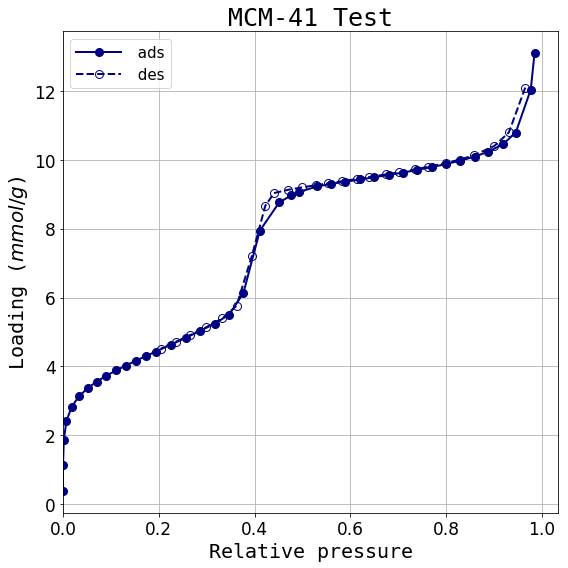
\includegraphics[width=0.5\linewidth]{printinfo}
    \caption{Resulting graph}\label{appx:pyg:print_info}
\end{figure}

\section{Information about materials chosen for reproducibility study}

\begin{table}[H]
	\centering
    \caption{Summary of ``ideal'' material surface areas referenced.}
	\begin{tabular}{lcll}
		\toprule
	    \textbf{Material}
        & \textbf{\ce{N2} accessible \gls{BET} Surface Area (\si{\metre^2\per\gram})} 
        & \textbf{Source} \\
		\midrule
        CuBTC        & 1909 & simulation~\cite{parkHowReproducibleAre2017}\\
        ZIF-8        & 1706 & simulation~\cite{fairen-jimenezOpeningGateFramework2011} \\
        MIL-101(Cr)  & 3892 & simulation~\cite{teoEvaluationCHCO2017} \\
        UiO-66(Zr)   & 1180 & simulation~\cite{parkHowReproducibleAre2017}\\
        IRMOF-1      & 3600 & simulation~\cite{pillaiUnderstandingGasAdsorption2015} \\
        IRMOF-3      & 2850 & experimental~\cite{nelsonSupercriticalProcessingRoute2009} \\
        IRMOF-8      & 4461 & simulation~\cite{pillaiUnderstandingGasAdsorption2015}\\
        MIL-100(Fe)  & 1928 & experimental~\cite{latrocheHydrogenStorageGiantPore2006} \\
        MIL-100(Cr)  & 1960 & simulation~\cite{hamonSeparationCO2CH42012} \\
        MIL-53(Cr)   & 1529 & simulation~\cite{jiaoStudiesGasAdsorption2017} \\
        MIL-53(Al)   & 1305 & simulation~\cite{jiaoStudiesGasAdsorption2017} \\
        MOF-14       & 1502 & simulation~\cite{chenInterwovenMetalOrganicFramework2001} \\
        COF-5        & 1590 & experimental~\cite{cotePorousCrystallineCovalent2005} \\
        MIL-68(Al)   & 1430 & simulation~\cite{yangProbingAdsorptionPerformance2012} \\
        Zn-MOF-74    & 1380 & simulation~\cite{linForceFieldDevelopmentElectronic2014} \\
        COF-10       & 2080 & experimental~\cite{coteReticularSynthesisMicroporous2007} \\
        \bottomrule
	\end{tabular}%
	\label{appx:pyg:tbl:materials}
\end{table}%


\bibliographystyle{unsrtnat}
\bibliography{backmatter/biblio/bib}